% Chapter Template

\chapter{Methodology} % Main chapter title
The following chapter will describe the problem that investigated in this work, the model adjustments and definitions,
the methods and the tools used to do so.

\label{chap:methodology} % Change X to a consecutive number; for referencing this chapter elsewhere, use \ref{ChapterX}

%----------------------------------------------------------------------------------------
%	SECTION 1
%----------------------------------------------------------------------------------------

\section{Problem definition}
\label{sec:problemDef}
%The goal of modeling is always to invent a model that is capable of correctly reproducing past and reliably predicting 
%future events. The latter is often very difficult, since it is necessary to correctly understand the dynamics of a
%complex system and then implement these dynamics in the form of a program, algorithm or method.\newline

%\par
The previous work of \cite{Rastogi} investigated the SEIRD model on a 2d-grid of Germany. In his work he simulated
all five groups of the SEIRD model for seven cities in Germany. This proved that the model itself is functional and
in principle capable of reproducing and predicting the dynamic of the COVID-19 pandemic or other pandemic/endemic events. \newline

\par
The goal of this work was to better understand the performance of the model in a smaller scale environment and to improve
the quality of the results. Hesse (Germany) and its regions where chosen as a template for a new 2d-grid. To minimize the
propagation of error throughout the SEIRD groups, we decided to focus on optimizing the fist class individuals, the Susceptible (\B{S}) group.
In this context we tried to reproduce/predict real world data and upcoming trends. Additionally we focused on evaluating the
sensitivity of \B{S} to the two variables $\alpha$ and $q$.

%-----------------------------------
%	SECTION 2
%-----------------------------------
\section{Data acquisition and model adjustment}
The following section will explain the processes of data acquisition, issues and modifications of the SEIRD model,
in order to improve the quality of the results.

%-----------------------------------
%	SUBSECTION 1
%-----------------------------------
\subsection{Data acquisition}
\label{sec:datacoll}
In order to perform SEIRD simulations, it was necessary to gather precise real world data for as many of the five groups as possible.
The source for this data was the Github project \cite{Gehrcke}, which provided both the number of COVID-19 infections,
as well as the number of COVID-19 related deaths per region in Germany. The repository provides data based on the case/death
numbers published by the RKI (Robert Koch Institute) and the Risklayer GmbH. In this work the data based on the RKI publications
was used. The data format were cumulative case/death numbers per region per day.\newline

\par
The hospitalization rate of confirmed COVID-19 infected individuals, the average time till symptom onset, the average time till
hospitalization and the lethality rate case of an infection was taken from RKI publications \cite{RKIcov}. At the time of acquisition, these
numbers were only estimations based on the literature of the current date.\newline

\par
The population of each region in Hesse was taken from the website ``statistic.hessen.de''. The data was sourced from \cite{HessePop}
in the category ``Bef\"olkerung in Hessen 2017 bis 2020 nach Verwaltungsbezirk in Monaten''. The size of each region in Hesse
was taken from \cite{HesseSize}.

%-----------------------------------
%	SUBSECTION 2
%-----------------------------------
\subsection{SEIRD model adjustments}
\label{sec:SEIRDredef}
In order to reach the goals described in \hyperref[sec:problemDef]{section \ref*{sec:problemDef}}, we decided to alter
the definitions of the Exposed (\B{E}) and Infected (\B{I}) groups. Furthermore we decided to set the variable
$\kappa$ to 1, effectively removing the option of exposed individuals to recover without developing symptoms. These
changes were done for two major reasons:\newline

\par
First, data availability proved to be an issue. The problem being, that the number of infected in the
collected data set only includes individuals where the COVID-19 pathogen could be isolated or that were tested positive
with a polymerase chain reaction (PCR) or antigen test\cite{RKIcase}. However,
these tests are usually conducted, if an individual is experiencing symptoms of sickness. This means, that individuals, that do
not experience symptoms were (for the most part) not represented in the collected data. In addition, it was difficult to estimate
the ratio between infected individuals that experience symptoms and individuals that do not experience symptoms. This made it
even harder make realistic assumptions, on which bases the original data could be modified to account for this phenomenon.\newline

\par
The second reason for these changes is a better representation of the actual disease history of COVID-19. Many infections
between susceptible and exposed individuals happen, before the exposed develop symptoms. While sick individuals can infect others many
days after symptom onset, about halve of all transmissions are pre-symptomatic \cite{casey2021presymptomatic} and that symptom onset generally
reduces transmission rates due to isolation measures\cite{RKIcov}.

\par
Based on this information, we did not allow for direct recovery from the model and redefined redefined the \B{E} and \B{I} groups as follows.
\begin{enumerate}[label=$\bullet$]
	\item \B{Exposed (E)}: Group of individuals that are infected with the virus and will develop symptoms in the upcoming
		days. Individuals are contagious during this time and contribute to infections of susceptibles.
	\item \B{Infected (I)}: Group of individuals that has experienced symptoms. Individuals are mostly not contagious anymore
		and isolate themself/are isolated until recovery or death.
\end{enumerate}

Of course these assumptions are not fully representative of the real world dynamics of COVID-19 disease spreading. However, based on
the information described prior, we think that these changes improve the overall accuracy of the model and the interpretation of real world data.

%----------------------------------------------------------------------------------------
%	SECTION 2
%----------------------------------------------------------------------------------------

\section{Experimental setup and pre-simulation work}
The following section will describe the assumptions made based on the previous explanations, the generation of a suitable data set and
the pre-processing of the newly created data.


%-----------------------------------
%	SUBSECTION 1
%-----------------------------------
\subsection{Assumptions}
Based on the information that was gathered, we made a set of assumptions in order to derive our experimental data from the raw data.
These assumptions are as follows.

\begin{enumerate}
	\item The average time for an exposed individual to develop symptoms is 6 days.
	\item After symptom development, an individual begins self isolation and does not contribute to new infections. It transitions to the \B{I} group.
	\item The average time for a symptomatic individual (\B{I} group) to lose most of its symptoms and contagiousness is about 10 days. This was defined as
		transition to the recovered (R) state.
	\item The average time between symptom onset and death was about 11 days during the first infection wave in Germany. This was
		defined as transition to the diseased (D) state.
	\item Based on points \B{3.} and \B{4.} we estimated a transition time from \B{E} to either \B{R} or \B{D} of 10 days. Using the
		average of 10.5 days was not possible, since only one data point per day was available.
\end{enumerate}


%-----------------------------------
%	SUBSECTION 2
%-----------------------------------
\subsection{Data pre-processing}
Since the raw data was cumulative, the number of individuals in each group at time point $t$ were defined as follows:

\begin{align}
	S(t) &= N - i(t+6)\\
	E(t) &= i(t+5) - i(t)\\
	I(t) &= i(t) - i(t-10)\\
	R(t) &= i(t-10) - d(t)\\
	D(t) &= d(t)
\end{align}

\par
Where $N$ represents the total number of individuals living in a specific region of Hesse at the beginning of the pandemic, $i(t)$
represents the cumulative number of infected individuals at time $t$ and $d(t)$ represents the cumulative number of deceased
individuals at time $t$. These calculations were done for each region, time point and group.\newline

We chose to simulate the time frame between 1\I{st} of September 2020 and the 15{th} of November 2020 (a time frame of 76 days). These
data points were chosen, since no significant policy changes regarding protective measures against COVID-19 infections
(mask mandates, isolation periods, store closures)  were made during this time in Germany. Thus hopefully providing a more stable system
with hard to predict variables. Additionally, this time frame was before other COVID-19 variants were first observed in
Germany\cite{RKIvariants}. It can therefore be assumed, that only the original CODIV-19 strain from Wuhan was contributing to infections.\newline

Each group was calculated for each day in each region. For the first day of simulation (day 0), the percentage of each group at that
point in time was calculated. These values were used as the starting point for all simulations.


%-----------------------------------
%	SUBSECTION 2
%-----------------------------------
\subsection{Generation of 2d-grid of Hesse}
For the simulation, a 2d-grid of Hesse was created using the program ProMesh4. The grid was manually drawn and consisted
of 1075 vertices and 3049 edges, from which 1975 faces (triangular volumes) were constructed and was divided into 26 regions,
representing the 26 autonomous regions of Hesse. The geometry and properties of the grid (also called mesh in the context of computational simulation)
make it unstructured. A visual representation of the grid and an exemplary
image of the original geography of Hesse are shown in \hyperref[fig:2d-grid]{Figure \ref*{fig:2d-grid}}.

%That means, that vertices can be positioned and connected arbitrarily. This method provides more flexibility then 
%\textcolor{red}{ADD FINITE VOLUME EXPLANATION?!?}

\begin{figure}
	\begin{center}
		\begin{subfigure}[b]{0.4\textwidth}
			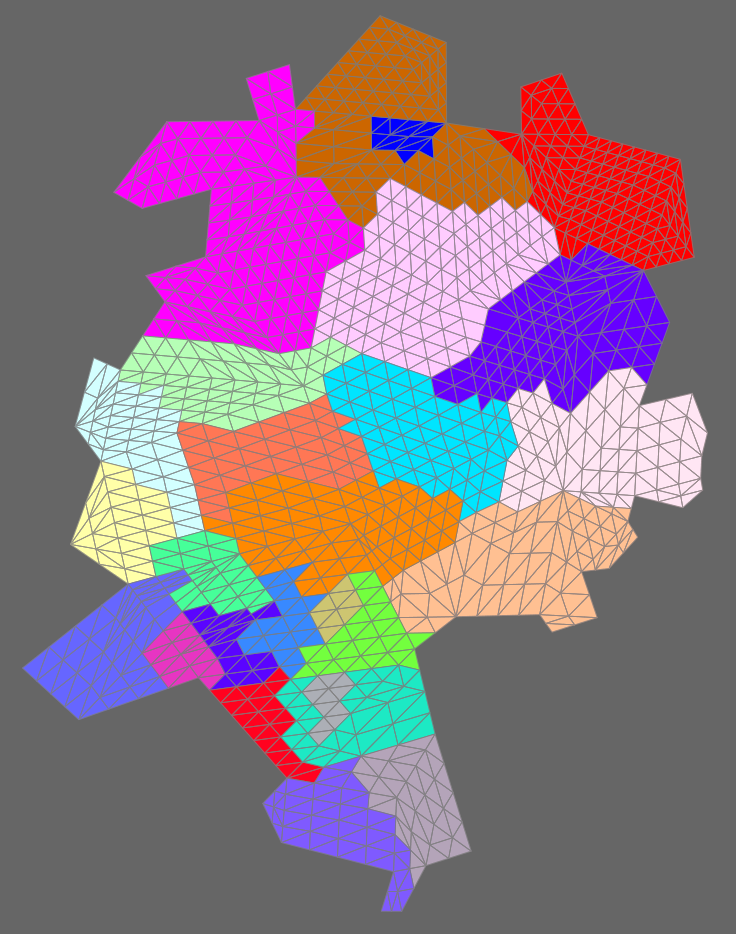
\includegraphics[width=\textwidth]{./figures/grid.png}
		\end{subfigure}
		% ---------------------
		\begin{subfigure}[b]{0.4\textwidth}
			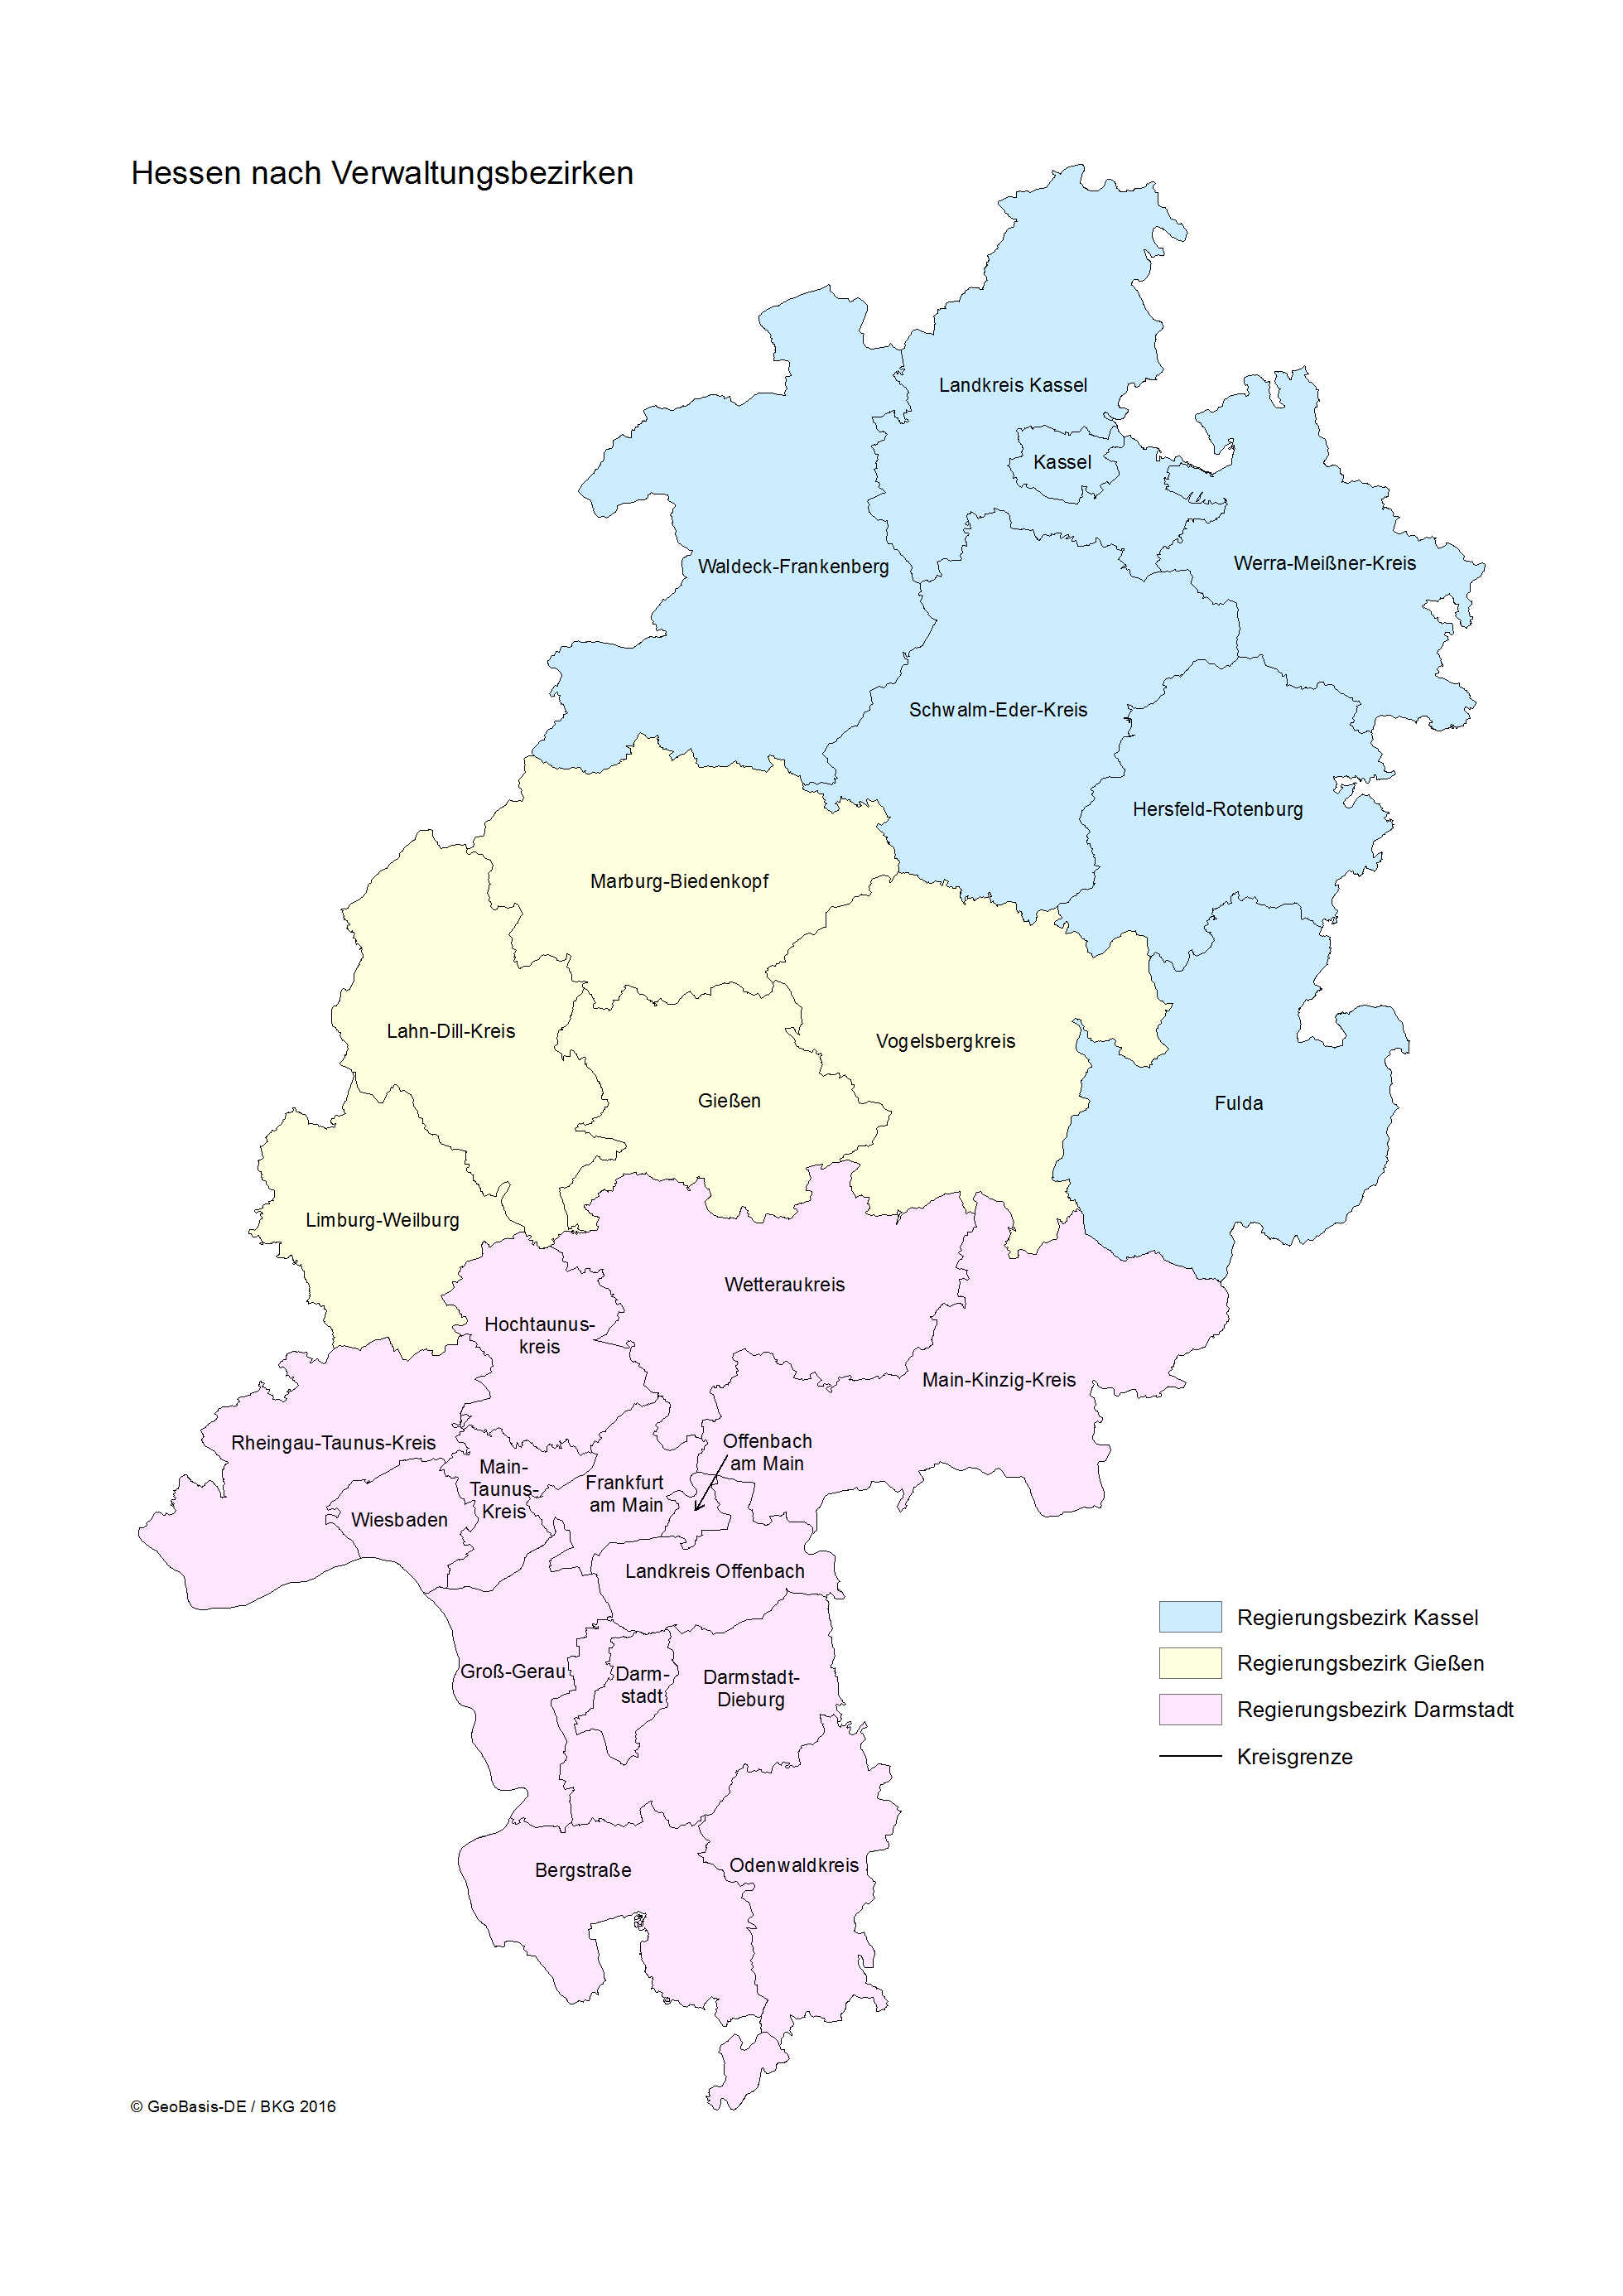
\includegraphics[width=\textwidth]{./figures/Hessen.png}
		\end{subfigure}
	\end{center}
	\caption{2d-grid of the region of Hesse. The grid consists of 1075 vertices, 3049 edges and 1975 faces.
		Each color on the grid represents a different region within Hesse. An image of Hesse is shown
		for better comparability\cite{HesseImage}.}
	\label{fig:2d-grid}
\end{figure}


%----------------------------------------------------------------------------------------
%	SECTION 3
%----------------------------------------------------------------------------------------

\section{SEIRD simulation}

\subsection{Inherited SEIRD model implementation}
The experiments of this work were  performed using the model implementation previously established in and kindly provided by
Rastogi et al.\cite{Rastogi}. The code provided included a functional implementation of the UG4 'EpidemicsRunner', as well as
the epidemics\_app folder used for  the previously mentioned project. The code was manly lua based and served as a base
for modifications and additional features added during this work. Changes and additions included both streamlining the simulation process, as
well as setting up the simulation experiments used to generate the results. The base file used to run the SEIRD simulation was epidemics.lua,
which was originally written by Prof. Gabriel Wittum and Dr. Arne N\"agel, and later modified by Devansh Rastogi and Tristan Scheidemann.
The previously mentioned lua files serve as a platform for the underlying UG4 framework. Commands issued in the lua files
are read and execute associated commands defined in UG4. 

\subsection{Process sequence of SEIRD simulations}
Simulations were performed as previously described by Rastogi et al.\cite{Rastogi}.
The implemented SEIRD simulation is based on an ugx file, that describes the geometry of the simulated regions. The file is provided
by the user and contains a number of vectors and edges. Vectors are grouped together to form regions, while edges describe possible
interactions between vectors that can be used to simulate migration between vectors. When the SEIRD model is started, starting conditions
defined in the lua code are applied to specific regions of the grid. From there the simulation is run for each
vector and the results are saved in an output file. If parameter optimization is performed, the results are then modified and processed
using the \I{ConstrainedOptimization} plugin (see \hyperref[sec:post_proc]{section \ref*{sec:post_proc}} for details).

%\subsection{LIMEX scheme}
% found new source, see notes.txt in /bachelor/thesis/

\subsection{Variable optimization}
For the process of optimizing the partial differential equation (PDE) problem, given by the model, two different solving methods
were used. The first method was a \I{Gauss-Newton} algorithm, the second was a \I{Particle Swarm Optimization} (PSO) algorithm.
During the experimental phase of the project both methods were used to investigate the questions answered in this work.
PSO was first used to roughly estimate possible target values, while \I{Gauss-Newton} was used to refine the previous findings.
Event though both methods yielded similar results in the end, all data presented in the result section of this work were created
using the \I{Gauss-Newton} algorithm. 

%----------------------------------------------------------------------------------------
%	SECTION 4
%----------------------------------------------------------------------------------------
\section{Data post-processing and variable optimization}
\label{sec:post_proc}
In order to optimize simulation results, the variables of the model equations had to be automatically adjusted based on
the loss value of the previous simulation. This section explains the steps that were undertaken to achieve this goal.

%-----------------------------------
%	SUBSECTION 1
%-----------------------------------
\subsection{Output-grid association}
The simulation results were output in the form of density values, associated with two coordinate positions ($x$ and $y$ on the
original grid). In order for the results to be processed properly, it was necessary to associate each of these
values with the correct region of the Hesse grid. To do, the program \I{geometry\_parser.lua} was written, which reads a config file,
parses and saves the positional information of each vertex in the grid and to which region it belongs. The program then compares the simulation results
with the parsed data and associates each result value with a region. Lastly the program \I{convert\_values.lua} is used to average the result values
for each region and time point, converts the average from densities to number of individuals per group and then saved the output in separate files.
One file per SEIRD group is created. The program was originally written by Devansh Rastogi and Tristan Scheidemann and later modified to
better suit the needs of this project. During simulations in which variables are optimized, the results are used to execute the program \I{ConstrainedOptimization}.


%-----------------------------------
%	SUBSECTION 2
%-----------------------------------
\subsection{Loss function}
In order to quantify the precision with which the simulation was able to reproduce the original data and optimize variables, the loss function $L$
was applied. Parameters of this function were the regions of Hesse $r$, a point in time $t$, the original data depending on
region and point in time $o(r_i,t_i)$ and the simulated data depending on region and point in time $s(r_i, t_i)$. Figure \ref*{eq:loss_newton}
shows the equation.

\textcolor{red}{do more mathematically correct}

\begin{align}
	L &= \sum_{r_0=0}^{25} \sum_{t_{0}=0}^{t} (o(r_i,t_i) - s(r_i,t_i))^{2}
	\label{eq:loss_newton}
\end{align}


%-----------------------------------
%	SUBSECTION 3
%-----------------------------------
\subsection{Variable optimization via \I{ConstrainedOptimization}}
The variables $\alpha$ and $q$ of the SEIRD system were optimized using the \I{ConstrainedOptimization} plugin for UG4\cite{Scheidemann}.
The plugin was used to optimize these variables using both the \I{Gauss-Newton} algorithm and PSO.

%Step sizes for individual time points were adjusted while using the \I{Gauss-Newton} algorithm. This was done via the Frank-Wolf algorithm\cite{Rastogi,frank-wolf}. %note add citaions


%-----------------------------------
%	SUBSECTION 4
%-----------------------------------
\subsection{Geometry sampling}
In order to better understand the sensitivity of the model for different variables, geometry sampling was done. This means that a set range for the
investigated variables was chosen and simulations were performed with randomly chosen values for said variables. After each run the total
loss of the simulation attempt was calculated and recorded. This data was then used to create a topographic map of the relation between variables
and the total loss of the simulation. In this work we observed the relation between loss and the variables $\alpha$ and $q$. These variables
were chosen, as they are the two variables influencing the observed group \B{S}. The program used for this task was the \I{geometry\_sampler}
provided in \I{ConstrainedOptimization}.


%----------------------------------------------------------------------------------------
%	SECTION 4
%----------------------------------------------------------------------------------------
\section{Data evaluation}
Data analysis of the simulation results was one of the main parts of this work. This section will highlight techniques and tools used during this process.

%-----------------------------------
%	SUBSECTION 1
%-----------------------------------
\subsection{Box plots}
Presenting the amount of data that was acquired in a compact and presentable way proved to be challenging. We decided to use box plots
as one of the main methods of presenting our data, as they convey a lot of key information to the reader without being to overwhelming.
Each box plot is made up of multiple elements. A Minimum, a Maximum, a first Quartile (Q1), a third Quartile (Q3), the Median and
the Outliers of the measurement. The Median is the middle value of the entire data set and lies between Q1 and Q3. Q1  is the Median 
between the lowest value of the data set and the Median of the entire data set. Thus 25\% of all data points are below and 75\% of
all data points are above Q1. Reversely Q3 is the Median value between the Median and the
highest value of the entire data set. Thus 75\% of all data ponints are below and 25\% of all data points are above Q3.
The difference between Q1 and Q3 is called the interquartile range (IQR). The Minimum and Maximum are
defined as $\text{Minimum} = Q1 - x*\text{IQR}$ and $\text{Maximum} = Q3 + x*\text{IQR}$, where $x$ was set to 1.5.
All values in the data set, that are located outside of the Minimum or Maximum are called Outliners and are represented as circles.
\hyperref[fig:boxplot]{Figure \ref*{fig:boxplot}} summarizes these definitions in an image.

\begin{figure}
	\begin{center}
		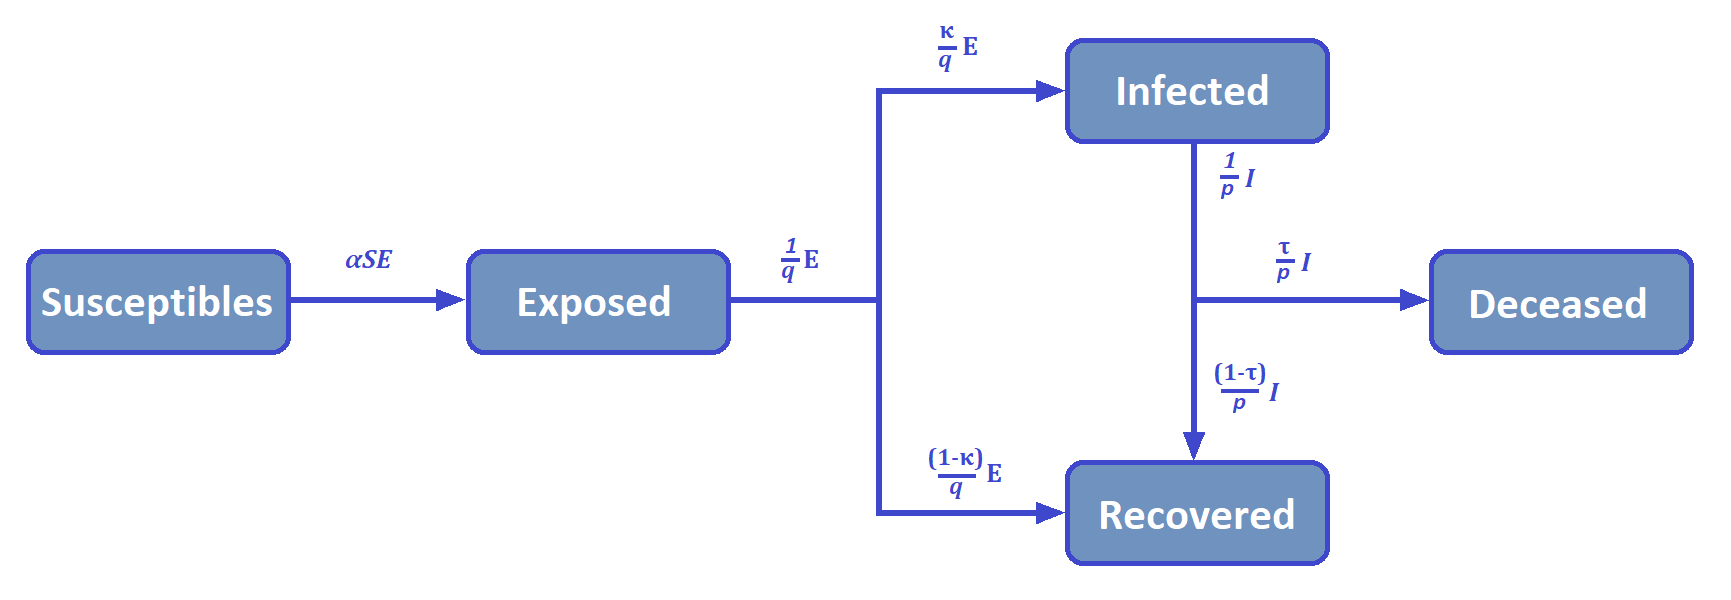
\includegraphics[width=0.75\textwidth]{./figures/SEIRD.png}
		\caption{Exemplary illustration of a box plot.
			}
		\label{fig:boxplot}
	\end{center}
\end{figure}


%-----------------------------------
%	SUBSECTION 2
%-----------------------------------
\subsection{Custom programs}
In order to present the results three custom programs were written. \I{deviation\_graph.py} was used to compare the data points of
individual regions. Graphs were created using matplotlib and numpy. Shortened data sets were extrapolated by fitting a polynomial
of degree three to the simulated data points. The resulting function was then extrapolated in order to highlight trends of the
analyzed data set. \I{deviation\_boxplot.py} was used to create box plots and \I{sensitivity\_plot} was used to visualize the
relation between $\alpha$, $q$ and the loss function in a three dimensional graph.
